\documentclass[11pt]{article}
\usepackage[margin=2.54cm]{geometry}
\usepackage[colorlinks,urlcolor=blue]{hyperref}
\usepackage{graphicx}

\title{CS 6140: Intermediate Report}
\author{Brian Kimmig, Jesus Zarate}
\date{}

\begin{document}

\maketitle

We began our analysis by looking at the genres. We will use a movies synopsis to predict what genres it is likely to be. In total, there were 26 unique genres. The frequency of genres varies a fair amount. Some genres occur less than 0.01\% of the time, while other occur close to 20\%. You can see the fraction of occurrence for each genre in Figure~\ref{fig:genre_fractions}. For our initial analysis we chose to cut out genres that occur less than 5\% of the time, this is shown by the red dotted line in Figure~\ref{fig:genre_fractions}. In the end we had the genres action, adventure, comedy, drama, romance and thriller. We will explore different cuts on this later if time permits.

\begin{figure}[h]
	\centering
		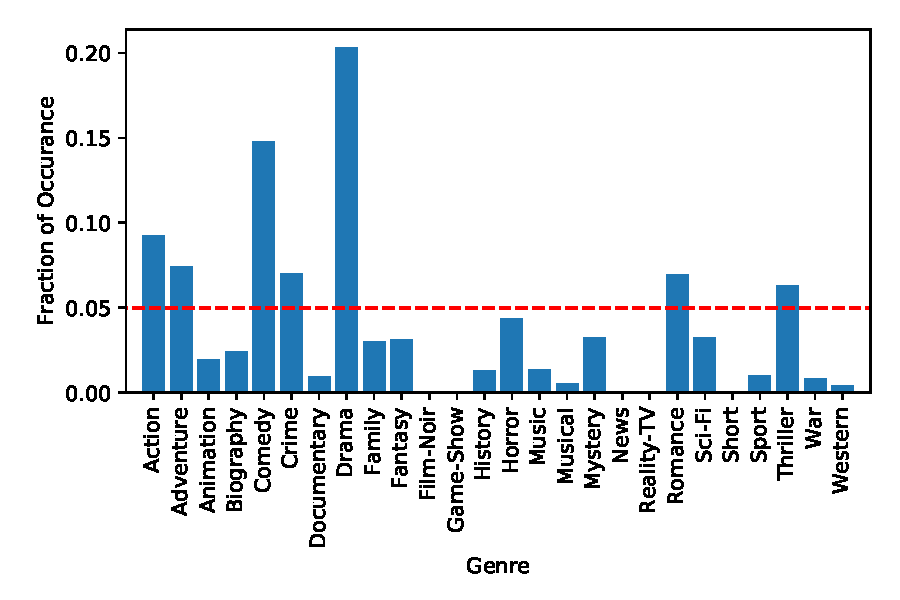
\includegraphics[width=0.5\textwidth]{genre_fractions_v2p0.pdf}
	\caption{The fraction of occurrence for each genre. The red dotted line represents the cut made to get the list of genres.}
	\label{fig:genre_fractions}
\end{figure}

Next, we set up a one hot encoding of our genres to build our classification labels. This is a matrix where the rows represent the movie and the column represents the genre. For each movie we put a 1 in the column that have the associated genre and zeros everywhere else.

Now we will discuss the creation of our feature matrix. The main idea used here is similar to $k$-grams but with some small differences. We will be using a method called {\it term frequency - inverse document frequency} \href{https://en.wikipedia.org/wiki/Tf%E2%80%93idf}{(TF-IDF)}. This looks at how frequently a term occurs in a document, in this case a movie synopsis, in combination with how frequently it occurs across all of the documents. This effectively down-weights the words that occur frequently in all documents. The term frequency is the number of times a given $k$-gram occurs in a document, and the inverse document frequency is the number of documents divided by the number of documents in which the $k$-gram occurs (the log of this is generally taken). First we create the matrix of term frequency counts represented in matrix form with $k$-grams as columns and each movie as a row. The inverse document frequency is a vector that contains the IDF for each $k$-gram. The final feature matrix is the multiplication each TF row by the IDF vector.

The next step is to get rid of common words. The first thing we did was try to eliminate stop words by just removing them from the columns of the matrix. \href{https://en.wikipedia.org/wiki/Stop_words}{Stop words} generally refer to the most common words in a language and will most likely not provide useful information in our feature matrix. However, removing stop words may not be good enough when we go to test with bi-grams or tri-grams. We may want to just eliminate the most common items that do not provide good information. Fortunately, TF-IDF can help with this, we can eliminate the words or $k$-grams that do not give us any information by making a cut on the inverse document frequency. However, it is easier to make this cut on just the document frequency, for example we may not want to keep term that occur in 80\% of the documents. This method seems to work just as well as removing stop words but with the added bonus of removing items with less information, especially in the different $k$-gram scenarios.

To this point, we have created the TF-IDF sparse matrix using single words and cut a cut on the document frequency at 70\%. This gave us a sparse matrix of shape $5029 \times 23988$ (rows by columns) with 234,707 elements. We then split this data into a train and test samples, with the test portion being 40\% of the data. We trained the basic out of the box \href{http://scikit-learn.org/stable/modules/generated/sklearn.ensemble.RandomForestClassifier.html}{Random Forest Classifier} from scikit-learn. 

To look at how well we predict each category we are using the \href{https://en.wikipedia.org/wiki/F1_score}{F1 score} which is the harmonic mean of precision and recall. The precision is the number of true-positives in your sample over the number of true and false positives. The recall is the number of true-positives over the number of true-positives and false-negatives. The best score in this scheme would be 1 and the worst would be 0.

After training on 60\% of the data we tested on the other 40\%. For each genre, Table \ref{tab:f1scores} shows the F1 scores. The features used for this classification include single words and a document frequency cut of 70\%. We obtain an average F1 score across all genres of 0.50. For this pass it is clear that the classification does better with the genres that occurs more frequently.

\begin{table}[h]
	\label{tab:f1scores}
\begin{center}
	\begin{tabular}{| l | l |}
		\hline
		Genre & F1-Score \\
	  	\hline			
	  	Action & 0.31 \\
	  	Adventure & 0.20 \\
	  	Comedy & 0.51 \\
	  	Crime & 0.23 \\
	  	Drama & 0.70 \\
	  	Romance & 0.10 \\
	  	Thriller & 0.11 \\
	  \hline  
	\end{tabular}
\end{center}
	\caption{The F1 scores for the prediction of each genre.}
\end{table}

The next steps will be to compare this with other feature sets. We plan to try bi-grams, tri-grams, and possibly mixes of the them. If time allows we may look into character level features. We also plan to mess with the document frequency threshold to see if limiting the features is more or less helpful.



\end{document}
